
\documentclass[xcolor=dvipsnames]{beamer} 
\usecolortheme[named=Blue]{structure} 
\usetheme[height=10.5mm]{Rochester} 
\setbeamertemplate{items}[ball] 
\setbeamertemplate{blocks}[rounded][shadow=true] 
\setbeamertemplate{navigation symbols}{} 
\usepackage{bm}
\usepackage{rotating}
\usepackage{graphicx}
\usepackage{multirow}
\usepackage{hyperref}
\usepackage{textcomp}
\usepackage{upquote}
\usepackage[absolute,overlay]{textpos}
\newenvironment{reference}[2]{%
  \begin{textblock*}{\textwidth}(#1,#2)
      \footnotesize\it\bgroup\color{red!50!black}}{\egroup\end{textblock*}}
%\graphicspath{ {/home/ben/PhD/Armidale_Updates/2014_03_14/Figures/} }
\begin{document}

\begin{frame} %1
% \frametitle{Addressing Common Challenges in Spatial Modeling of Ecologies and Environments}
%\begin{center}
\textbf{\huge Introduction to R}\\
a language and environment for statistical computing and graphics %
%\end{center}

\begin{figure}

\includegraphics[width = 0.35\textwidth]{/home/ben/Intro_to_R/Introductory_Slides_Source/Images/R_logo.png}
\end{figure}
\small Ben R. Fitzpatrick\\
\tiny PhD Candidate, Statistical Science, Mathematical Sciences School, Queensland University of Technology
\newline
\begin{columns}
\begin{column}{3cm}
\tiny 0000-0003-1916-0939
\end{column}
\begin{column}{3cm}
\tiny github.com/brfitzpatrick/
\end{column}
\begin{column}{3cm}
\tiny @benrfitzpatrick
\end{column}
\end{columns}
\end{frame}



\begin{frame} 
\frametitle{What is R?}
\end{frame}

\begin{frame} 
\frametitle{Why Use R?}
\framesubtitle{R is Free in the Sense of Free Speach \& Free Beer}
\end{frame}

\begin{frame} 
\frametitle{Why Use R?}
\framesubtitle{R has many packages implementing a broad range of statistical analyses}

\begin{figure}
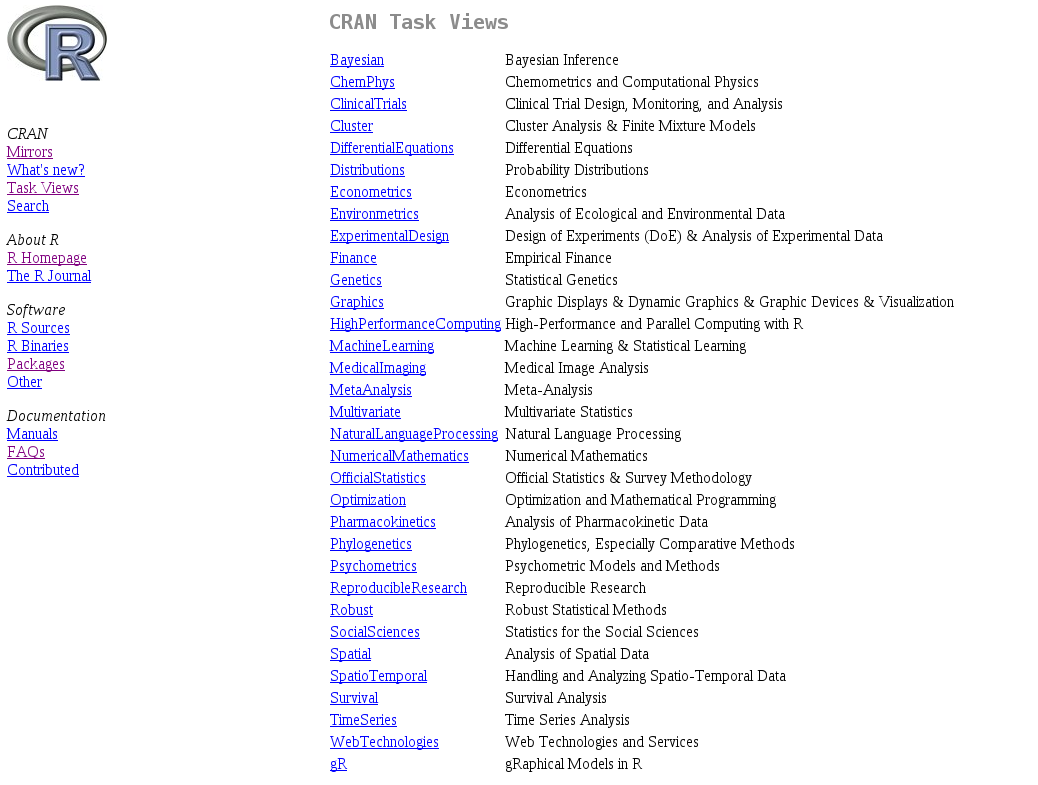
\includegraphics[height = 0.95\textheight]{/home/ben/Intro_to_R/Introductory_Slides_Source/Images/CRAN_Task_Views.png}
\end{figure}

\end{frame}

\begin{frame} 
\frametitle{Why Use R?}
\framesubtitle{R has powerful graphic authoring capabilities}

\begin{figure}
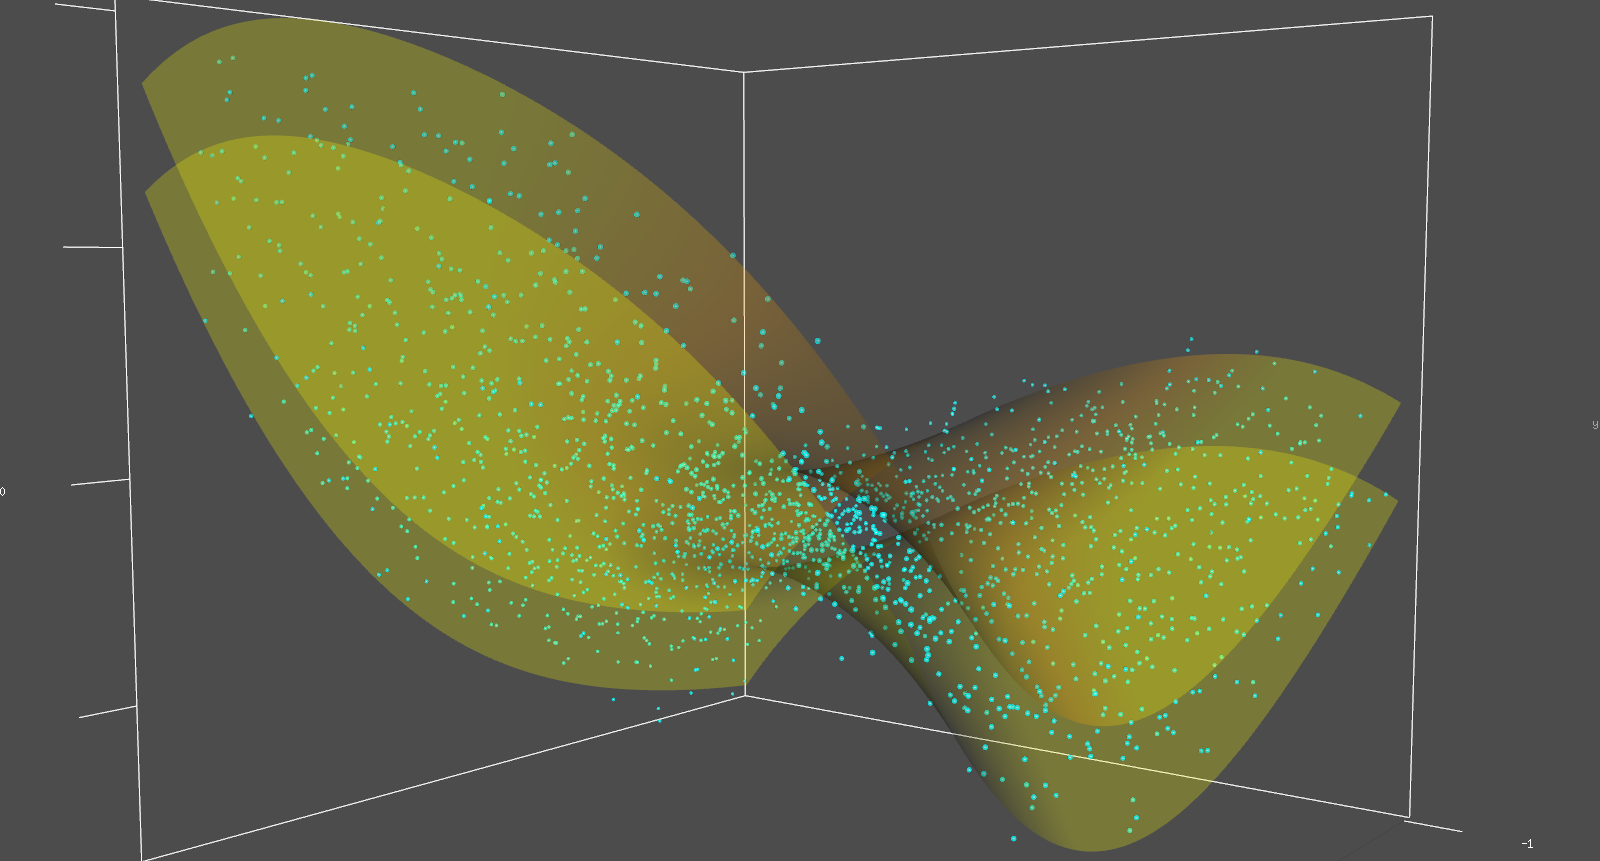
\includegraphics[width = 0.95\textwidth]{/home/ben/Intro_to_R/Introductory_Slides_Source/Images/179.png}
\end{figure}

\tiny 3D visualisation produced with the `rgl' R package

\end{frame}

\begin{frame} 
\frametitle{Why Use R?}
\framesubtitle{R is Popular with Large \& Steadily Growing User Base}


\end{frame}


\begin{frame} 
\frametitle{Why Use R?}
\framesubtitle{Popular}
\end{frame}



\begin{frame} 
\frametitle{Ways to Use R}
\begin{itemize}
\item via a termial on the command line
\item via the default clients for MS Windows \& Mac OS
\item via one of the many Integrated Development Environments \begin{itemize}
 \item RStudio
 \item Tinn-R
 \item Emacs Speaks Statistics \end{itemize}
\end{itemize}
\end{frame}

\begin{frame}
\frametitle{Ways to Use R:}
\framesubtitle{In a termial e.g. on MS Windows}
%\begin{figure}
%\includegraphics[width = 0.35\textwidth]{~/Presents_Intro_to_R/Introductory_Slides_Source/Images/R_Console_MacOS.png}
%\end{figure}
\end{frame}

\begin{frame}
\frametitle{Ways to Use R:}
\framesubtitle{In a termial e.g. on Mac OS}
\begin{figure}
\includegraphics[width = \textwidth]{/home/ben/Intro_to_R/Introductory_Slides_Source/Images/R_Console_MacOS.png}
\end{figure}
\end{frame}

\begin{frame}
\frametitle{Ways to Use R:}
\framesubtitle{In a termial e.g. on GNU+Linux}
\begin{figure}
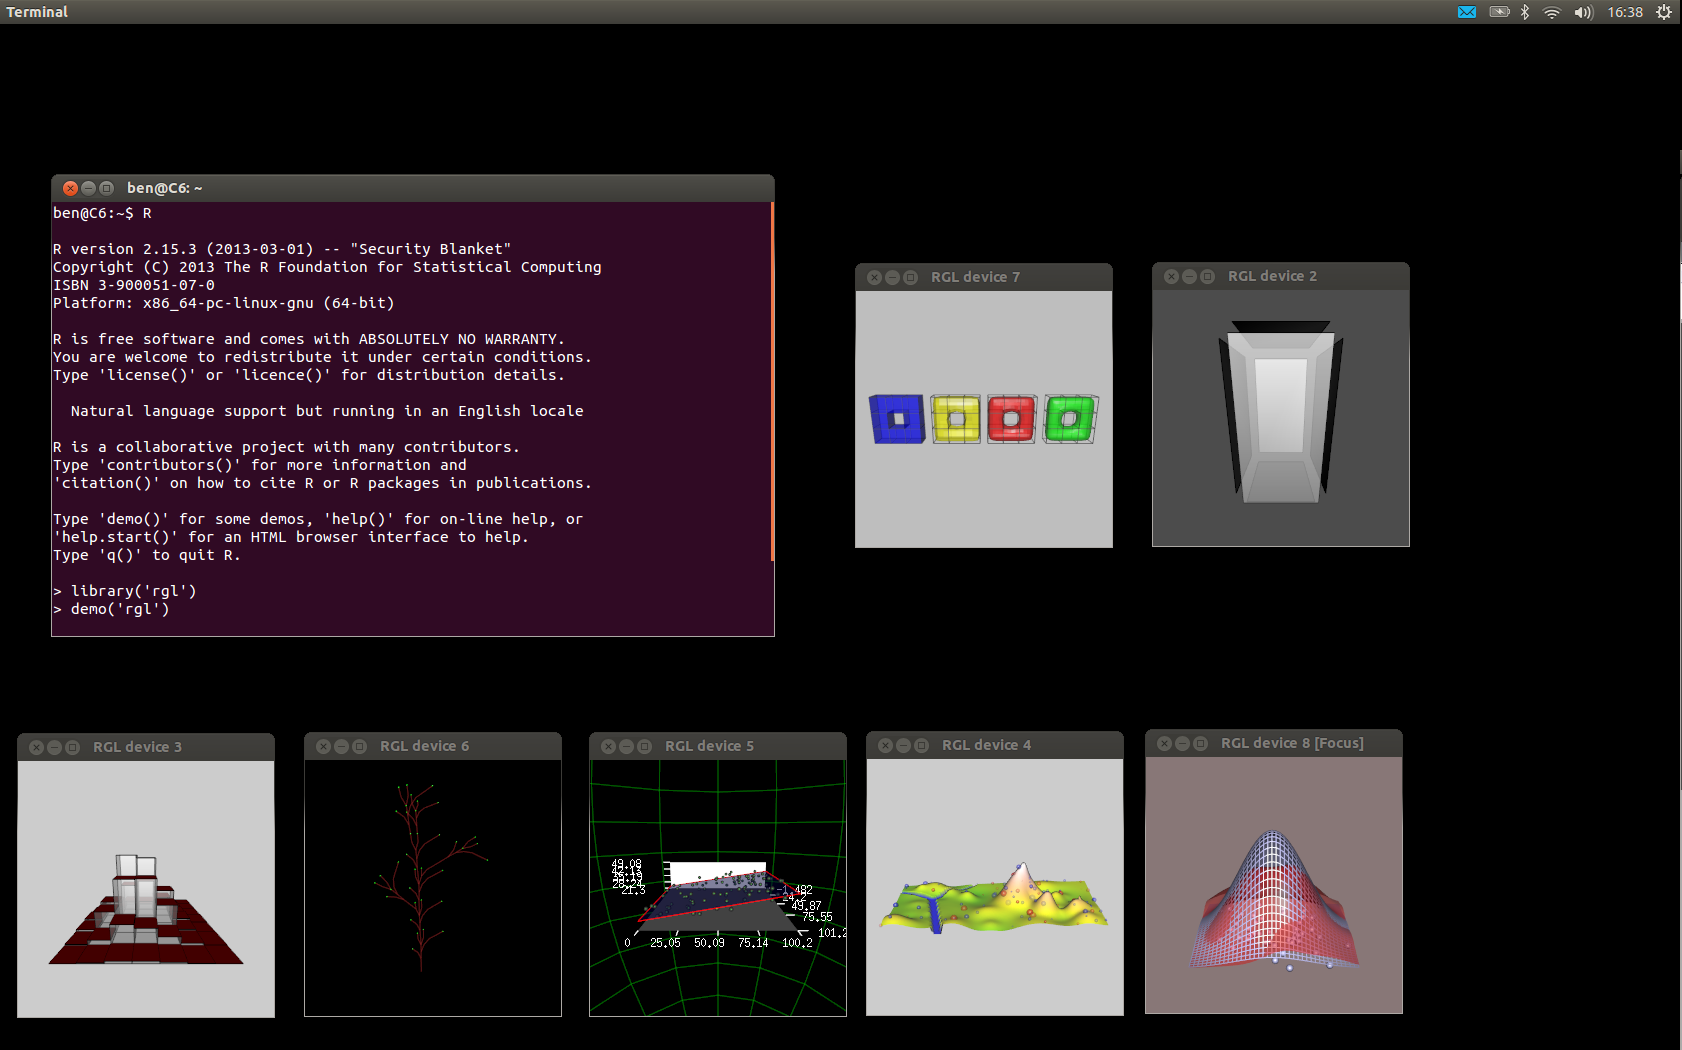
\includegraphics[width = \textwidth]{/home/ben/Intro_to_R/Introductory_Slides_Source/Images/R_in_Ubuntu_Terminal_2.png}
\end{figure}
\end{frame}

\begin{frame}
\frametitle{Ways to Use R:}
\framesubtitle{Default Windows Client}
\begin{figure}
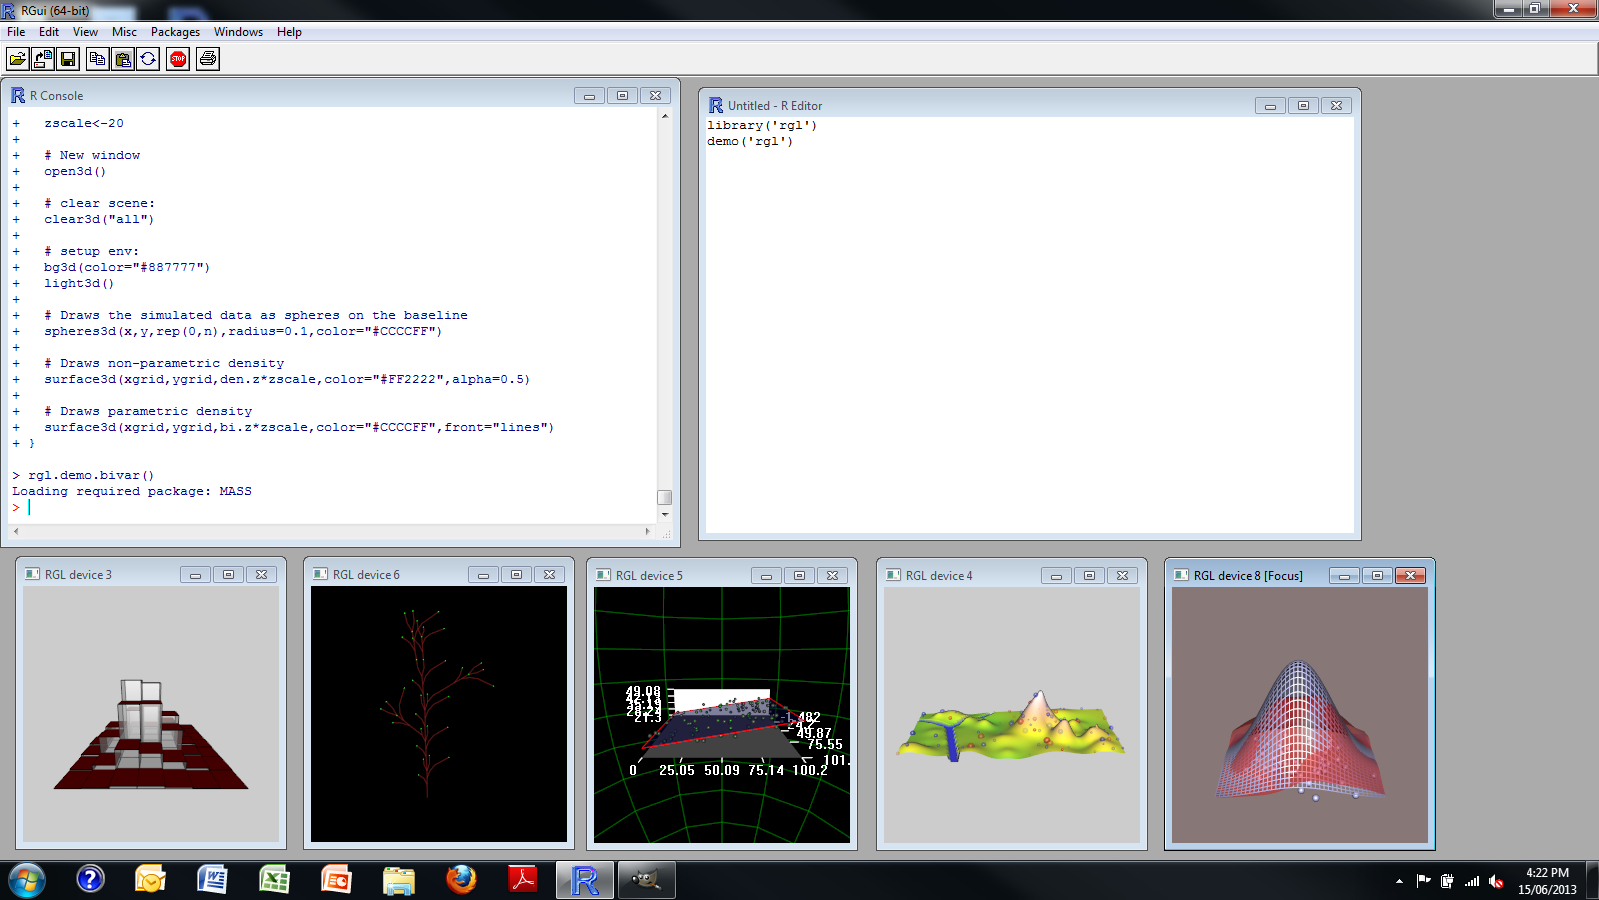
\includegraphics[width = \textwidth]{/home/ben/Intro_to_R/Introductory_Slides_Source/Images/R_on_Windows.png}
\end{figure}
\end{frame}

\begin{frame}
\frametitle{Ways to Use R:}
\framesubtitle{Tinn-R Integrated Development Environement}
\begin{figure}
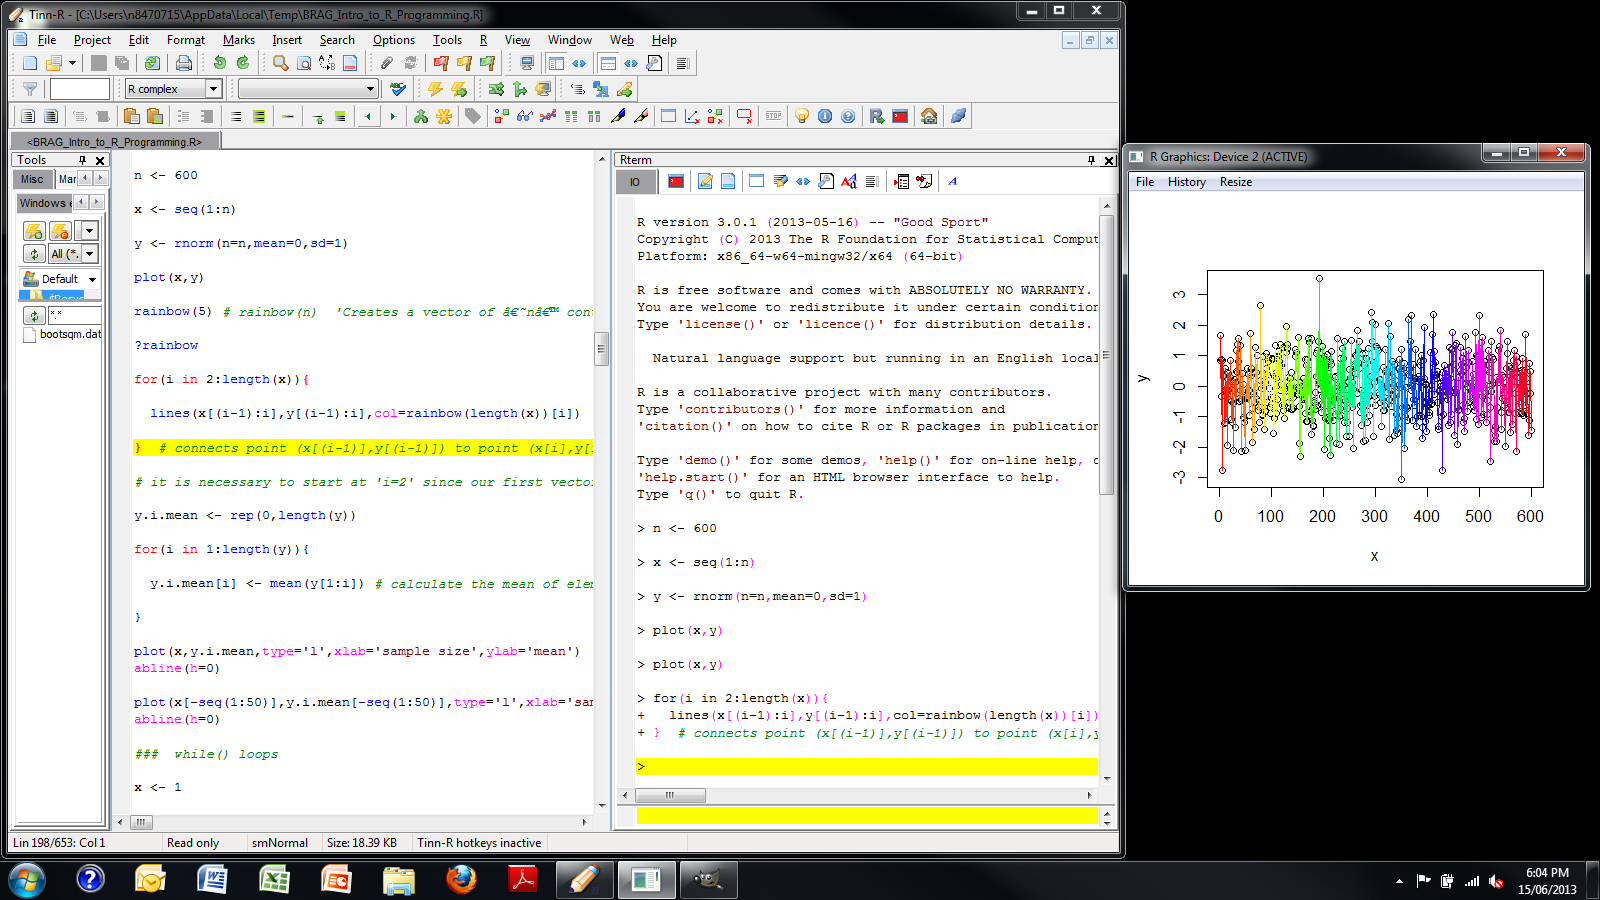
\includegraphics[width = \textwidth]{/home/ben/Intro_to_R/Introductory_Slides_Source/Images/TinnR.png}
\end{figure}
\end{frame}

\begin{frame}
\frametitle{Ways to Use R:}
\framesubtitle{Emacs Speaks Statistics Integrated Development Environement}
\begin{figure}
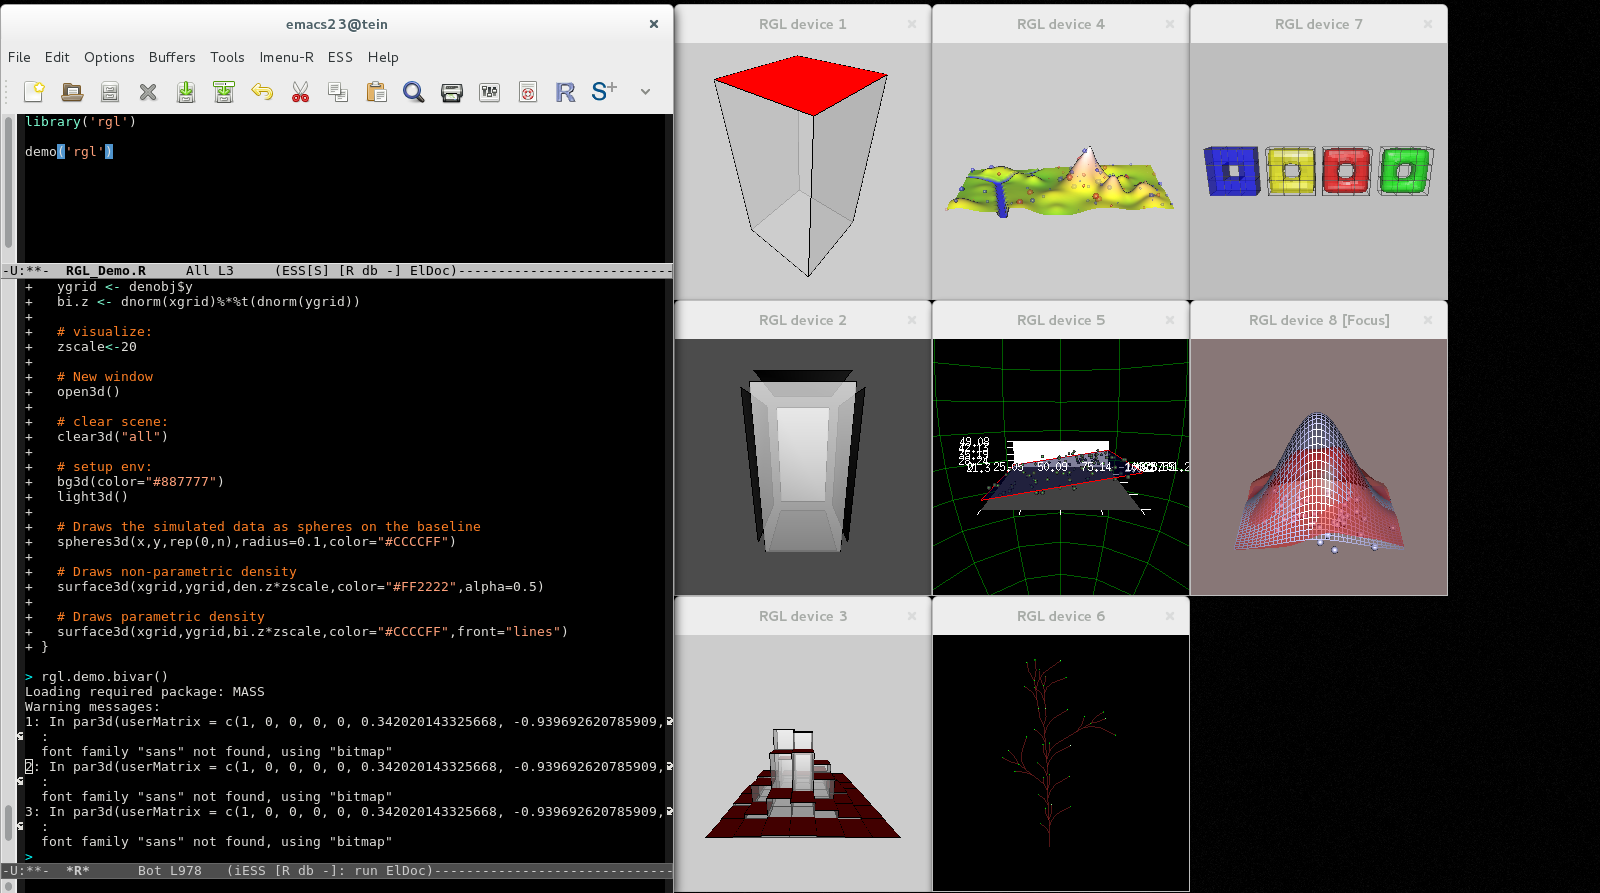
\includegraphics[width = \textwidth]{/home/ben/Intro_to_R/Introductory_Slides_Source/Images/R_ESS_Debian_GNU_Linux.png}
\end{figure}
\end{frame}

\begin{frame}
\frametitle{Ways to Use R:}
\framesubtitle{RStudio Integrated Development Environement}
\begin{figure}
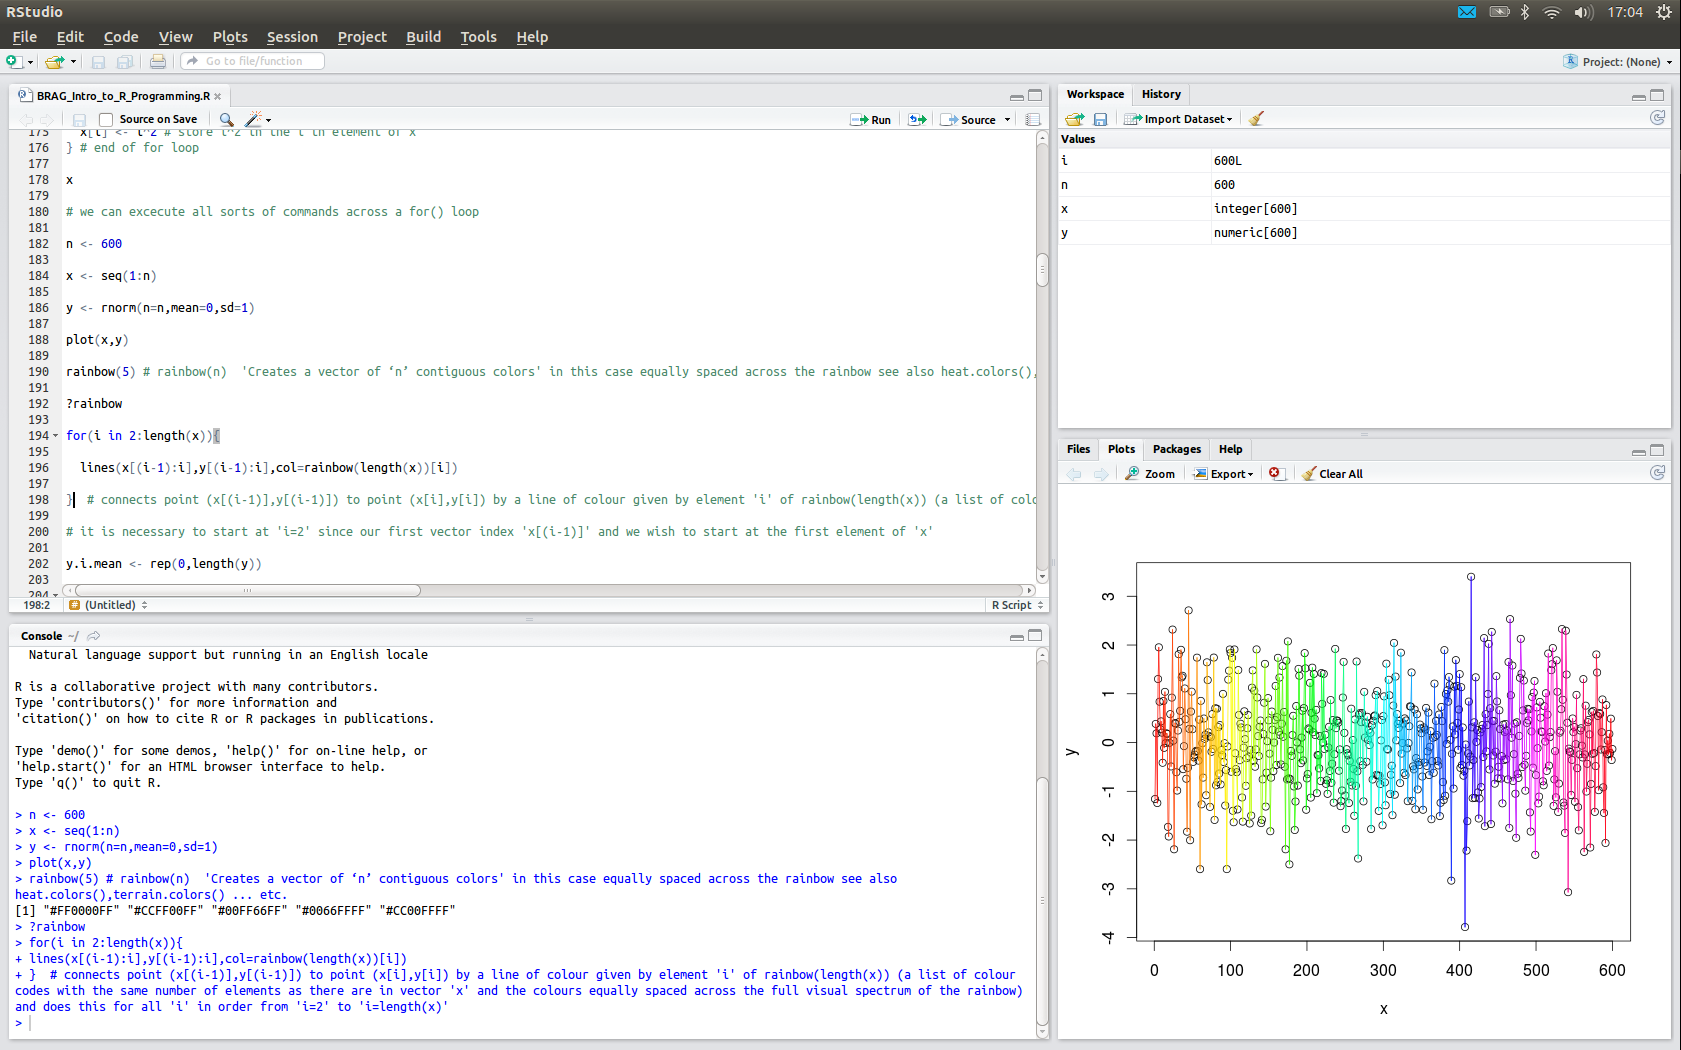
\includegraphics[width = \textwidth]{/home/ben/Intro_to_R/Introductory_Slides_Source/Images/RStudio_R.png}
\end{figure}
\end{frame}

\begin{frame}
\frametitle{For this course we'll use RStudio}
Because it's comparatively :...
\begin{itemize}
\item intuitive and easy to learn
\item feature rich
\item available for most major operating systems (MS Windows, Mac OS, various flavours of GNU+Linux)
\item interacts with Git for version control via GitHub
\end{itemize}

\end{frame}

\begin{frame}
\frametitle{If you're already familiar with R}
\frametitle{Feel free to use this time to pursue something that interests you}
You could
\begin{itemize}
\item Visit the GitHub directory for this course and pick a code file you like to start working through \url{https://github.com/brfitzpatrick/Intro_to_R}
\item See how far you can get through the incrementally harder maths/programming problems at \url{https://projecteuler.net/}
\item pursue your own project work
\end{itemize}
I'll need to focus on delivering the course but I'll try to check in with you peridocially throughout the next 2.5 days.
\end{frame}


\begin{frame} 
\frametitle{Image Credits}
R Foundation, from http://www.r-project.org - Originally from http://developer.r-project.org/Logo/Rlogo.svg, modified to simpler SVG format.
%
\end{frame}


\end{document}